\chapter{評価および考察}
\label{evaluation}

本章では,\ref{implementation}章で実装した本研究での提案手法の評価とその考察を述べる.

\section{評価手法}
\label{evaluation:method}

本実験システムの評価として,~\ref{approach:YotenForProblem}節で述べた要件に対して評価を行う.\\

本研究では,以下の三種類のHoneypotを設置する.\\
1. 広く利用されているSSHの低対話型Honeypot\\
2. 実際のShellには実装されているが,1.のHoneypotで未実装のコマンドを実装したHoneypot\\
3. 広く利用されている高対話型Honeypot\\

これ以降,1.の広く利用されているSSHの低対話型Honeypotのことを”純正の低対話型Honeypot” , 2.の実際のShellには実装されているが,1.のHoneypotで未実装のコマンドを実装したHoneypotのことを"修正済みの低対話型Honeypot" , 3.の広く利用されている高対話型Honeypotのことを"高対話型Honeypot"と呼ぶこととする.\\

以上3つの純正のHoneypot,修正済みのHoneypot,高対話型Honneypotのそれぞれで侵入ログを収集する.\\

また第3章の予備実験では,純正のHoneypotに実装されていないコマンドで悪意のある侵入者が使うようなコマンドを実装し,純正のHoneypotで取れた侵入者の実行コマンドログと,修正済みのHoneypotの侵入者の実行コマンドログを比較することで,修正済みのHoneypotの方がコマンドパターンとして多く収集できることを示した.\\
予備実験における収集ログの比較の概念図を図6に示す.

\begin{figure}[H]
    \centering
    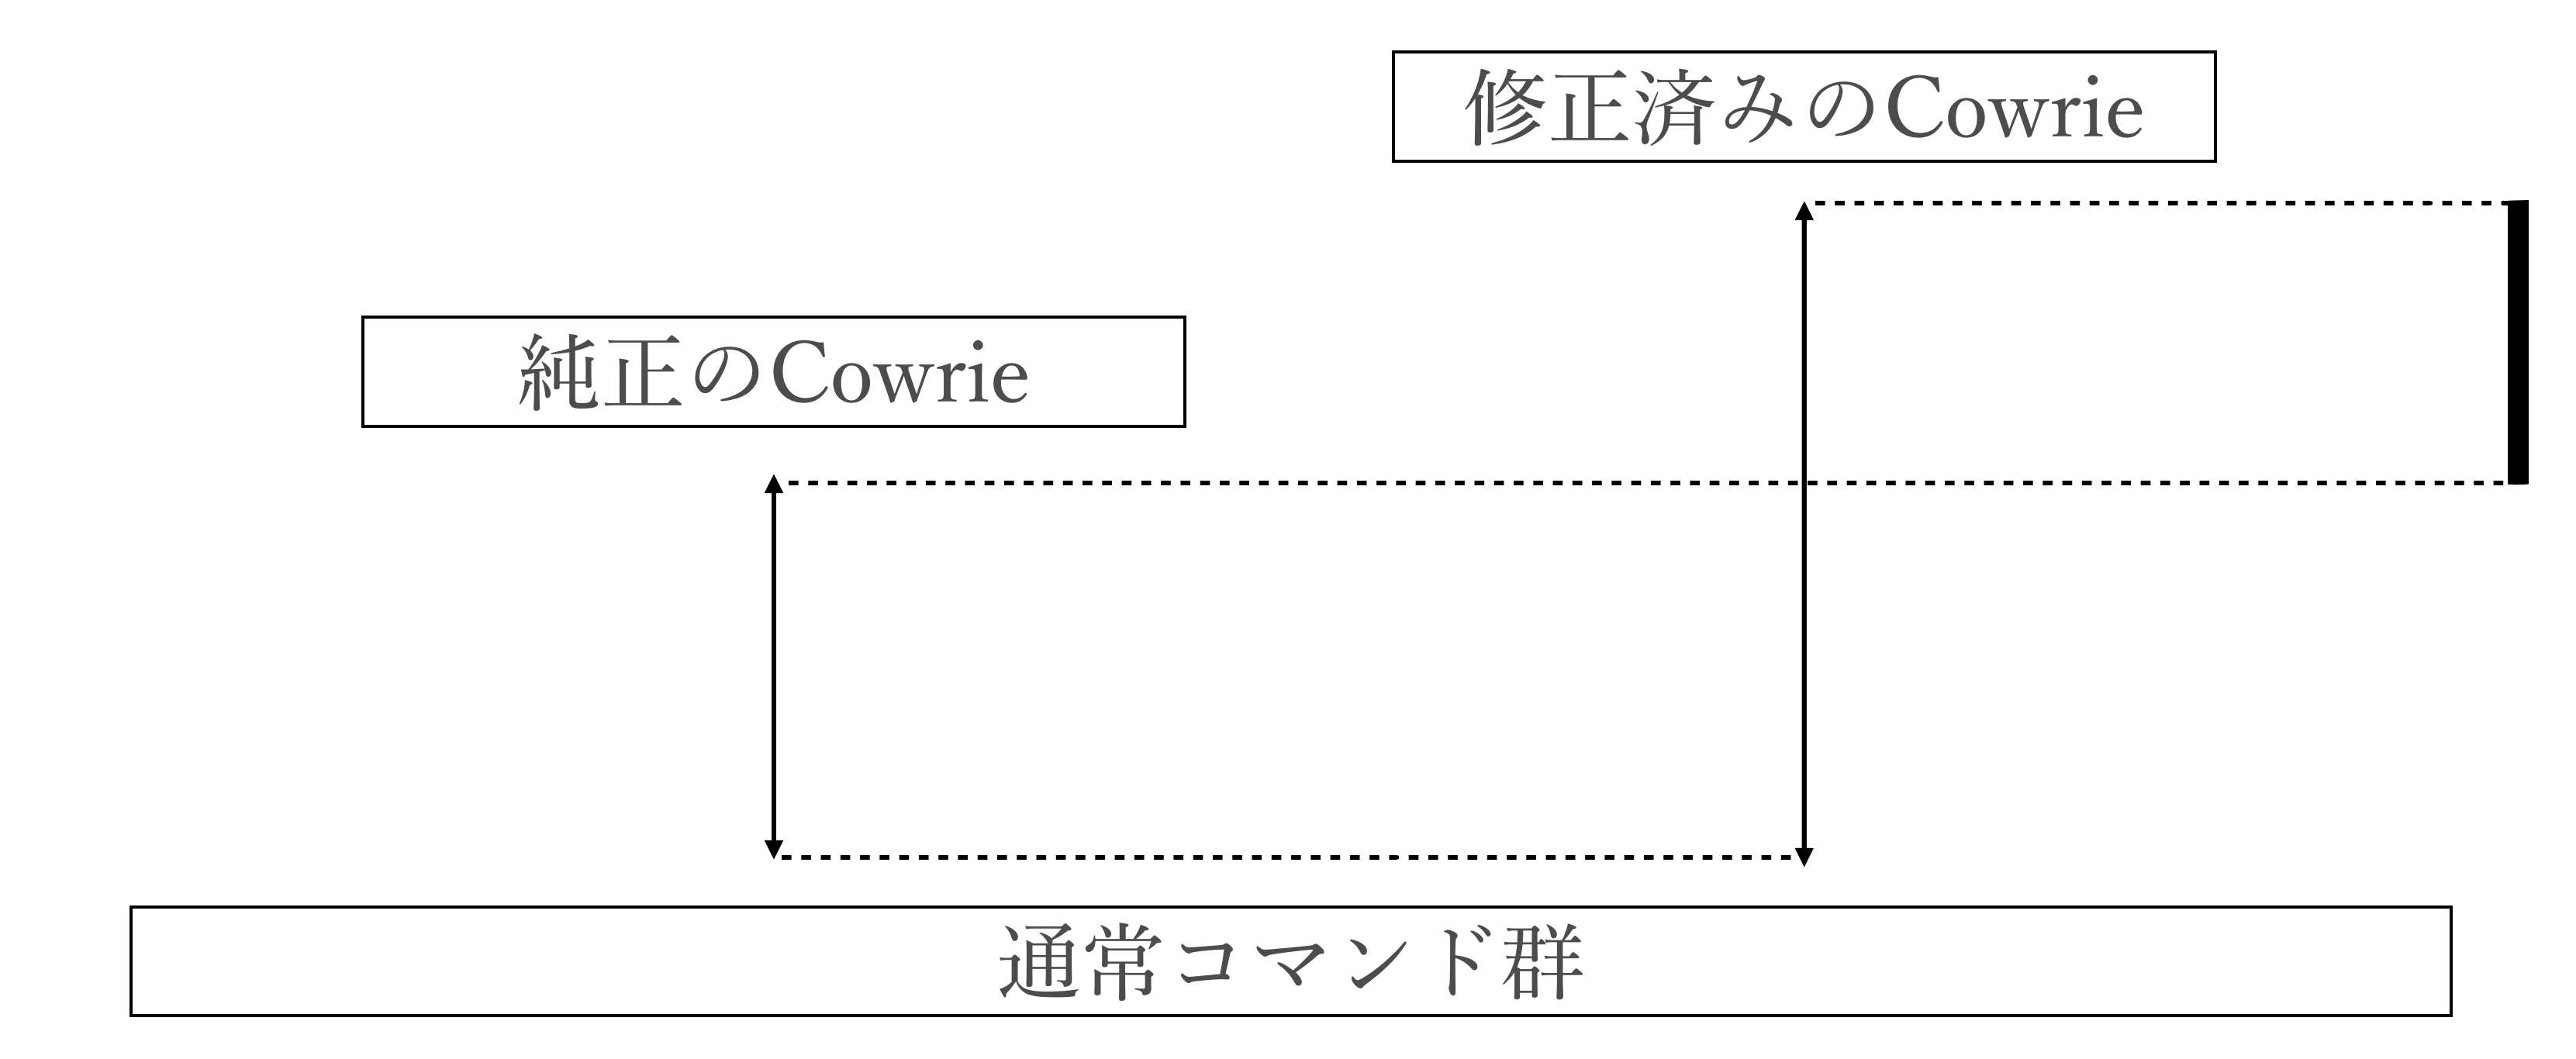
\includegraphics[width=1.0\textwidth]{figures/termhyoka.png}
    \caption{予備実験の評価の概念図}
    \label{fig:evo}
\end{figure}

この予備実験では評価として何の追加実装も施していないSSHの低対話型Honeypotで取れた侵入者の実行コマンドログと追加実装を施したSSHの低対話型Honeypotの侵入者の実行コマンドログとを比較したのに対して,本件研究の評価手法では,純正のHoneypotで取れた侵入者の実行コマンドログと修正済みのHoneypotの侵入者の実行コマンドログをと高対話型Honeypotの侵入者の実行コマンドログを比較することで,修正済みのHoneypotの侵入者の実行コマンドログが実際のShellの挙動にどれほど近似したのかを評価した.\\
予備実験における収集ログの比較の概念図を図7に示す.

\begin{figure}[H]
    \centering
    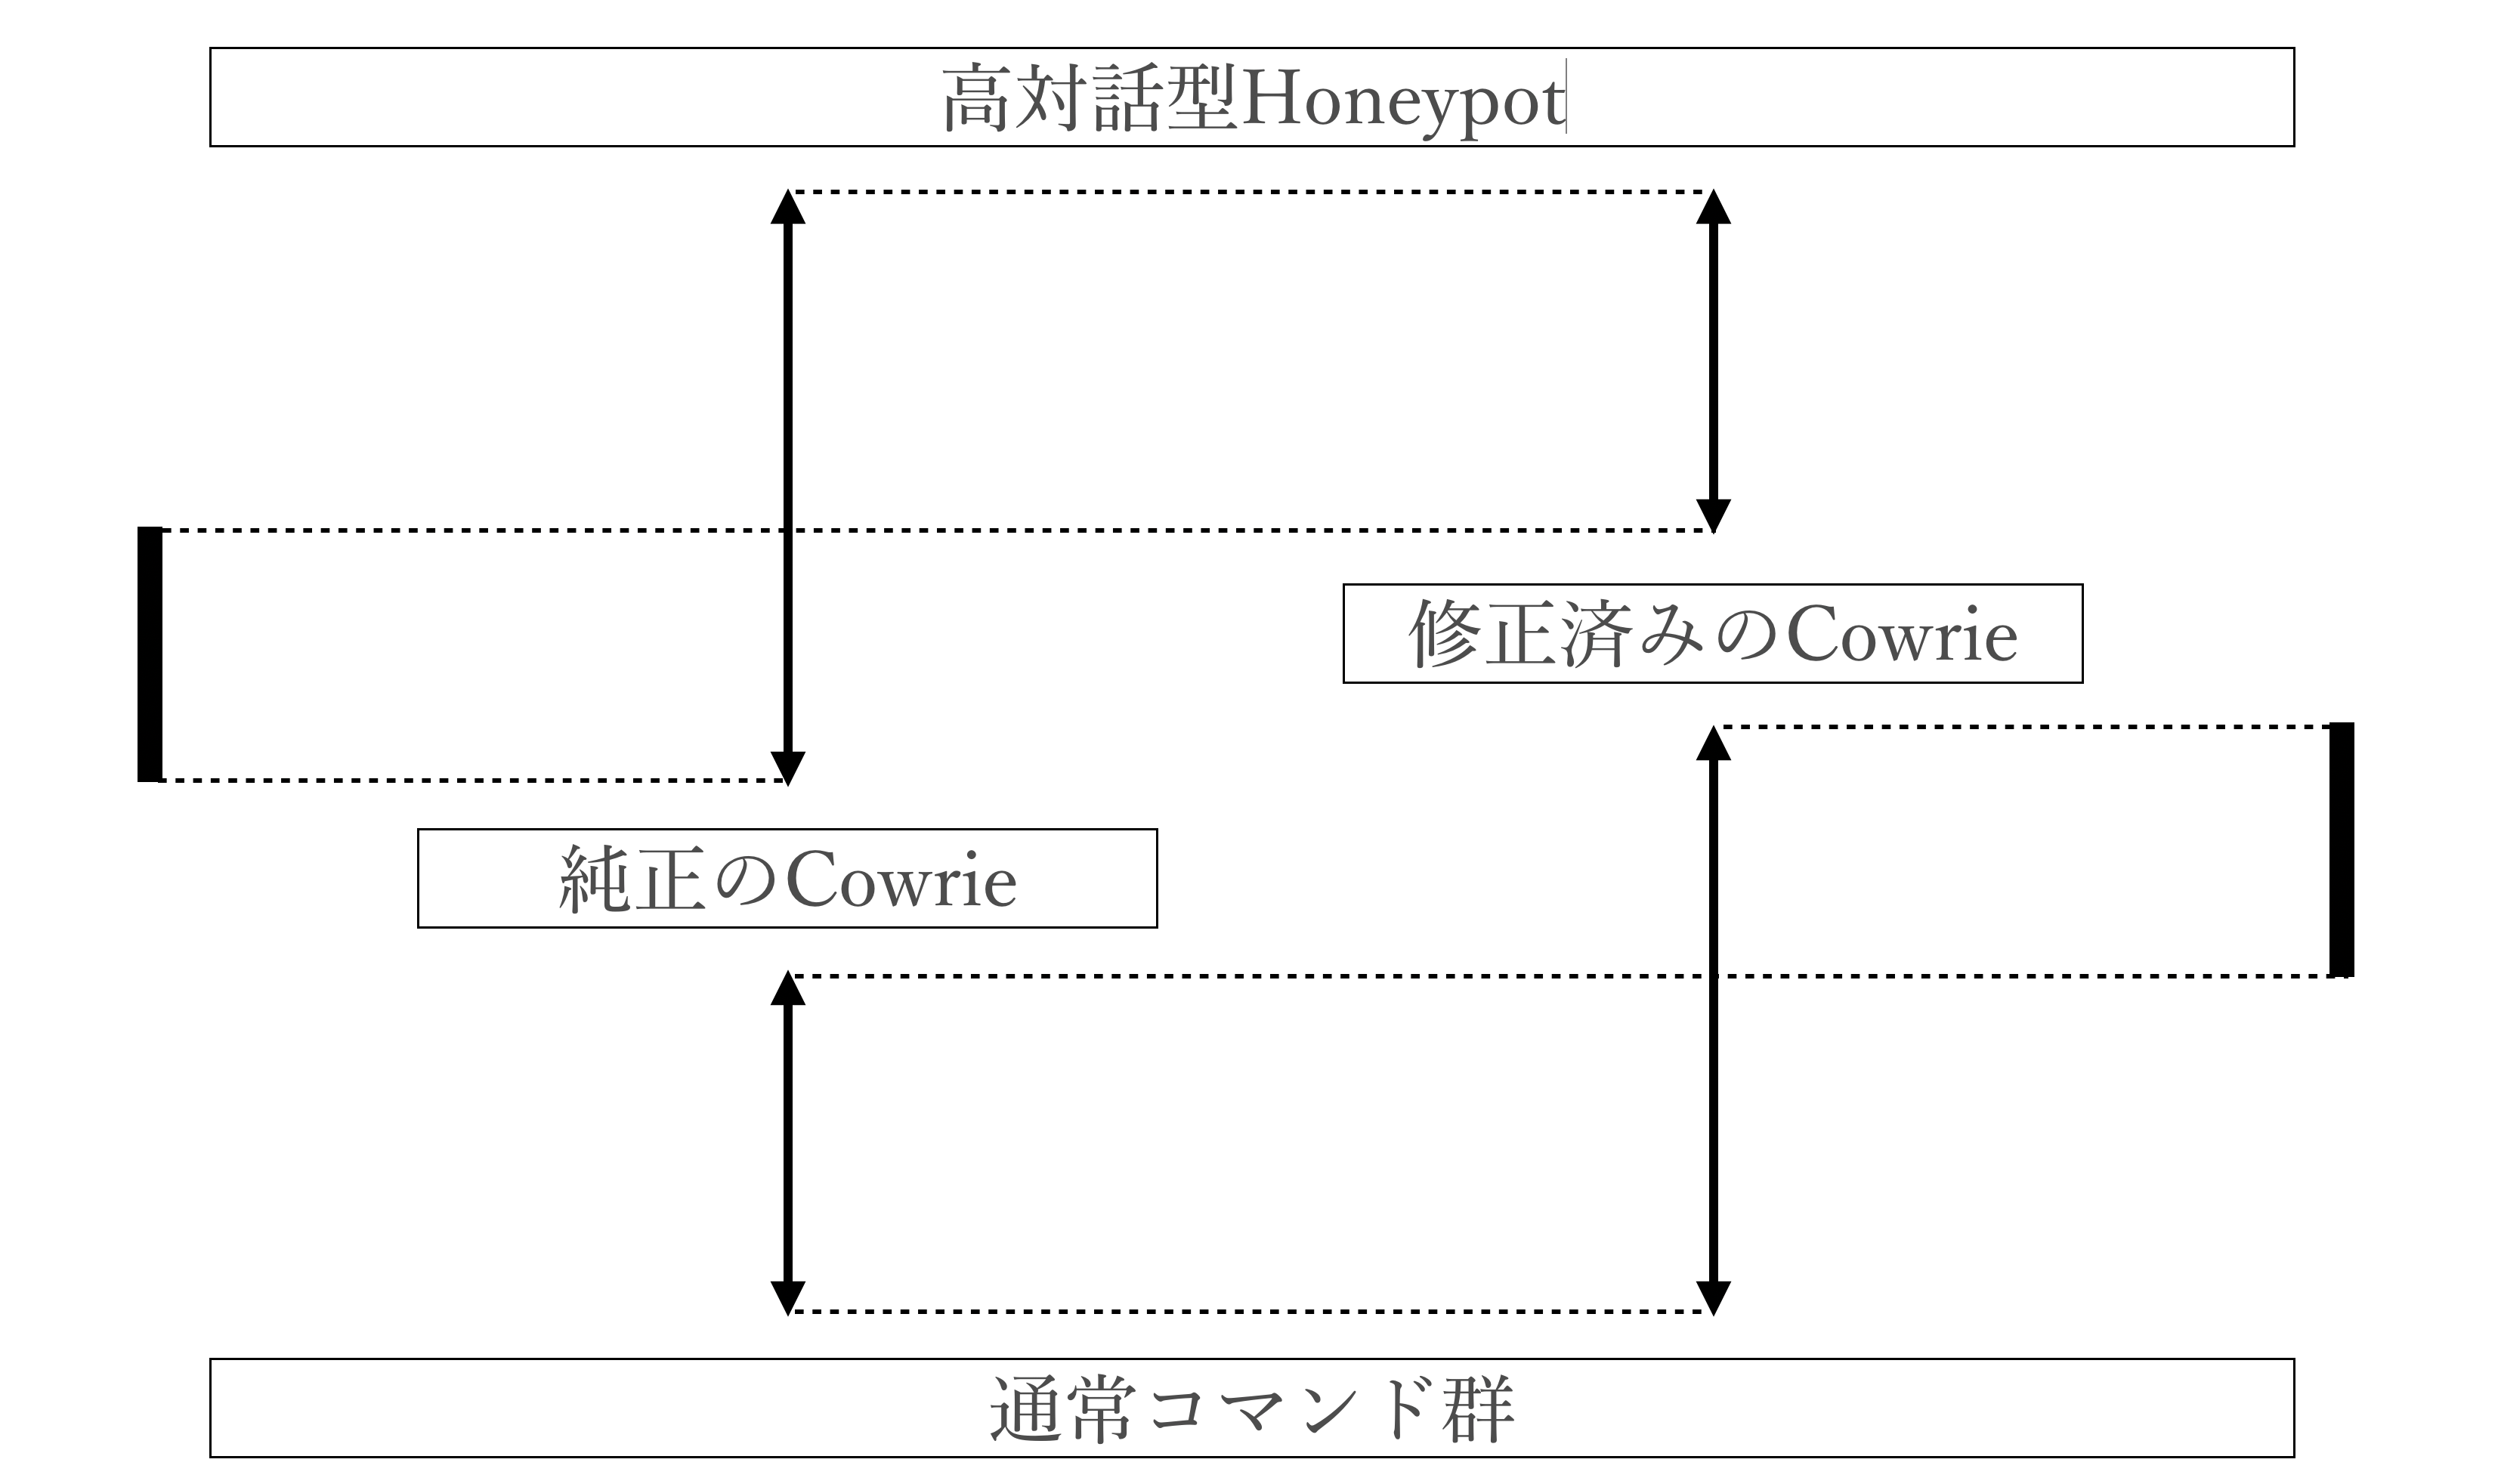
\includegraphics[width=1.0\textwidth]{figures/sotuhyoka.png}
    \caption{本研究の評価の概念図}
    \label{fig:evo}
\end{figure}

図6,と図7で示したようにして,取れた収集ログを比較することでいかに高対話型Honeypotに近似できたのか検証する.


\subsection{評価手法の実装}
\label{evaluation:impl}
純正の低対話型Honeypotで収集した侵入ログでskip-gramモデルの隠れ層の重みを学習させ(これをモデル1
とする),同様にして高対話型Honeypotで収集した侵入ログもskip-gramモデルの隠れ層の重みを学習させる(これをモデル2とする).次に修正済みのHoneypotで収集したログをセッション開始からセッション終了までに打たれたコマンドごとに(以降これを1セッションごとと呼ぶ)モデル1とモデル2のそれぞれに入力していき,出力された数値aを活性化関数としてソフトマックス関数をかけることで,0≦a≦1の範囲を取るようにし確率的な数値として出力することでスコアリングを行う.このため入力に対して多数存在する出力を全てを合計すると1になる.
純正の低対話型Honeypotや高対話型Honeypotの収集ログをモデル化する際、入力層として収集ログのコマンドの入力に対してそのコマンドの周辺のコマンドを出力として与えることでこれを学習させる.\\
例えば3つのコマンドが打たれたとしたとしたものを以下のプログラム\,3に示す.

\vspace{5mm}
%\lstnewenvironment{mylisting}[1][]
%    {\lstset{
%        frame=single,
%        basicstyle=\ttfamily,
%        numbers=left,
%        numbersep=10pt,
%        tabsize=2,
%        extendedchars=true,
%        xleftmargin=17pt,
%        framexleftmargin=17pt,
%        #1
%    }
%}{}

\begin{mylisting}[language=sh,caption=3つの実行コマンドの例]
 $ uname
 $ free
 $ ps x
\end{mylisting}
\vspace{5mm}

モデルを構築する際には"free"コマンドを入力にした時に,出力として"uname"コマンド"ps"コマンドを用意しておくことで,freeが入力として与えられた時に他2つの出力される周辺のコマンドが出力する確率が高くなるようにする.また,実装としては周辺語をどこまで広げるのかはパラメータとしてwindow sizeで与えることができ,上記の例の周辺語は"1"であり,window sizeを"2"にすればモデル化する際に出力層に与えられる数は4つとなる.

以下の図8にモデル化のフローを示す.
\vspace{10mm}
\begin{figure}[H]
    \centering
    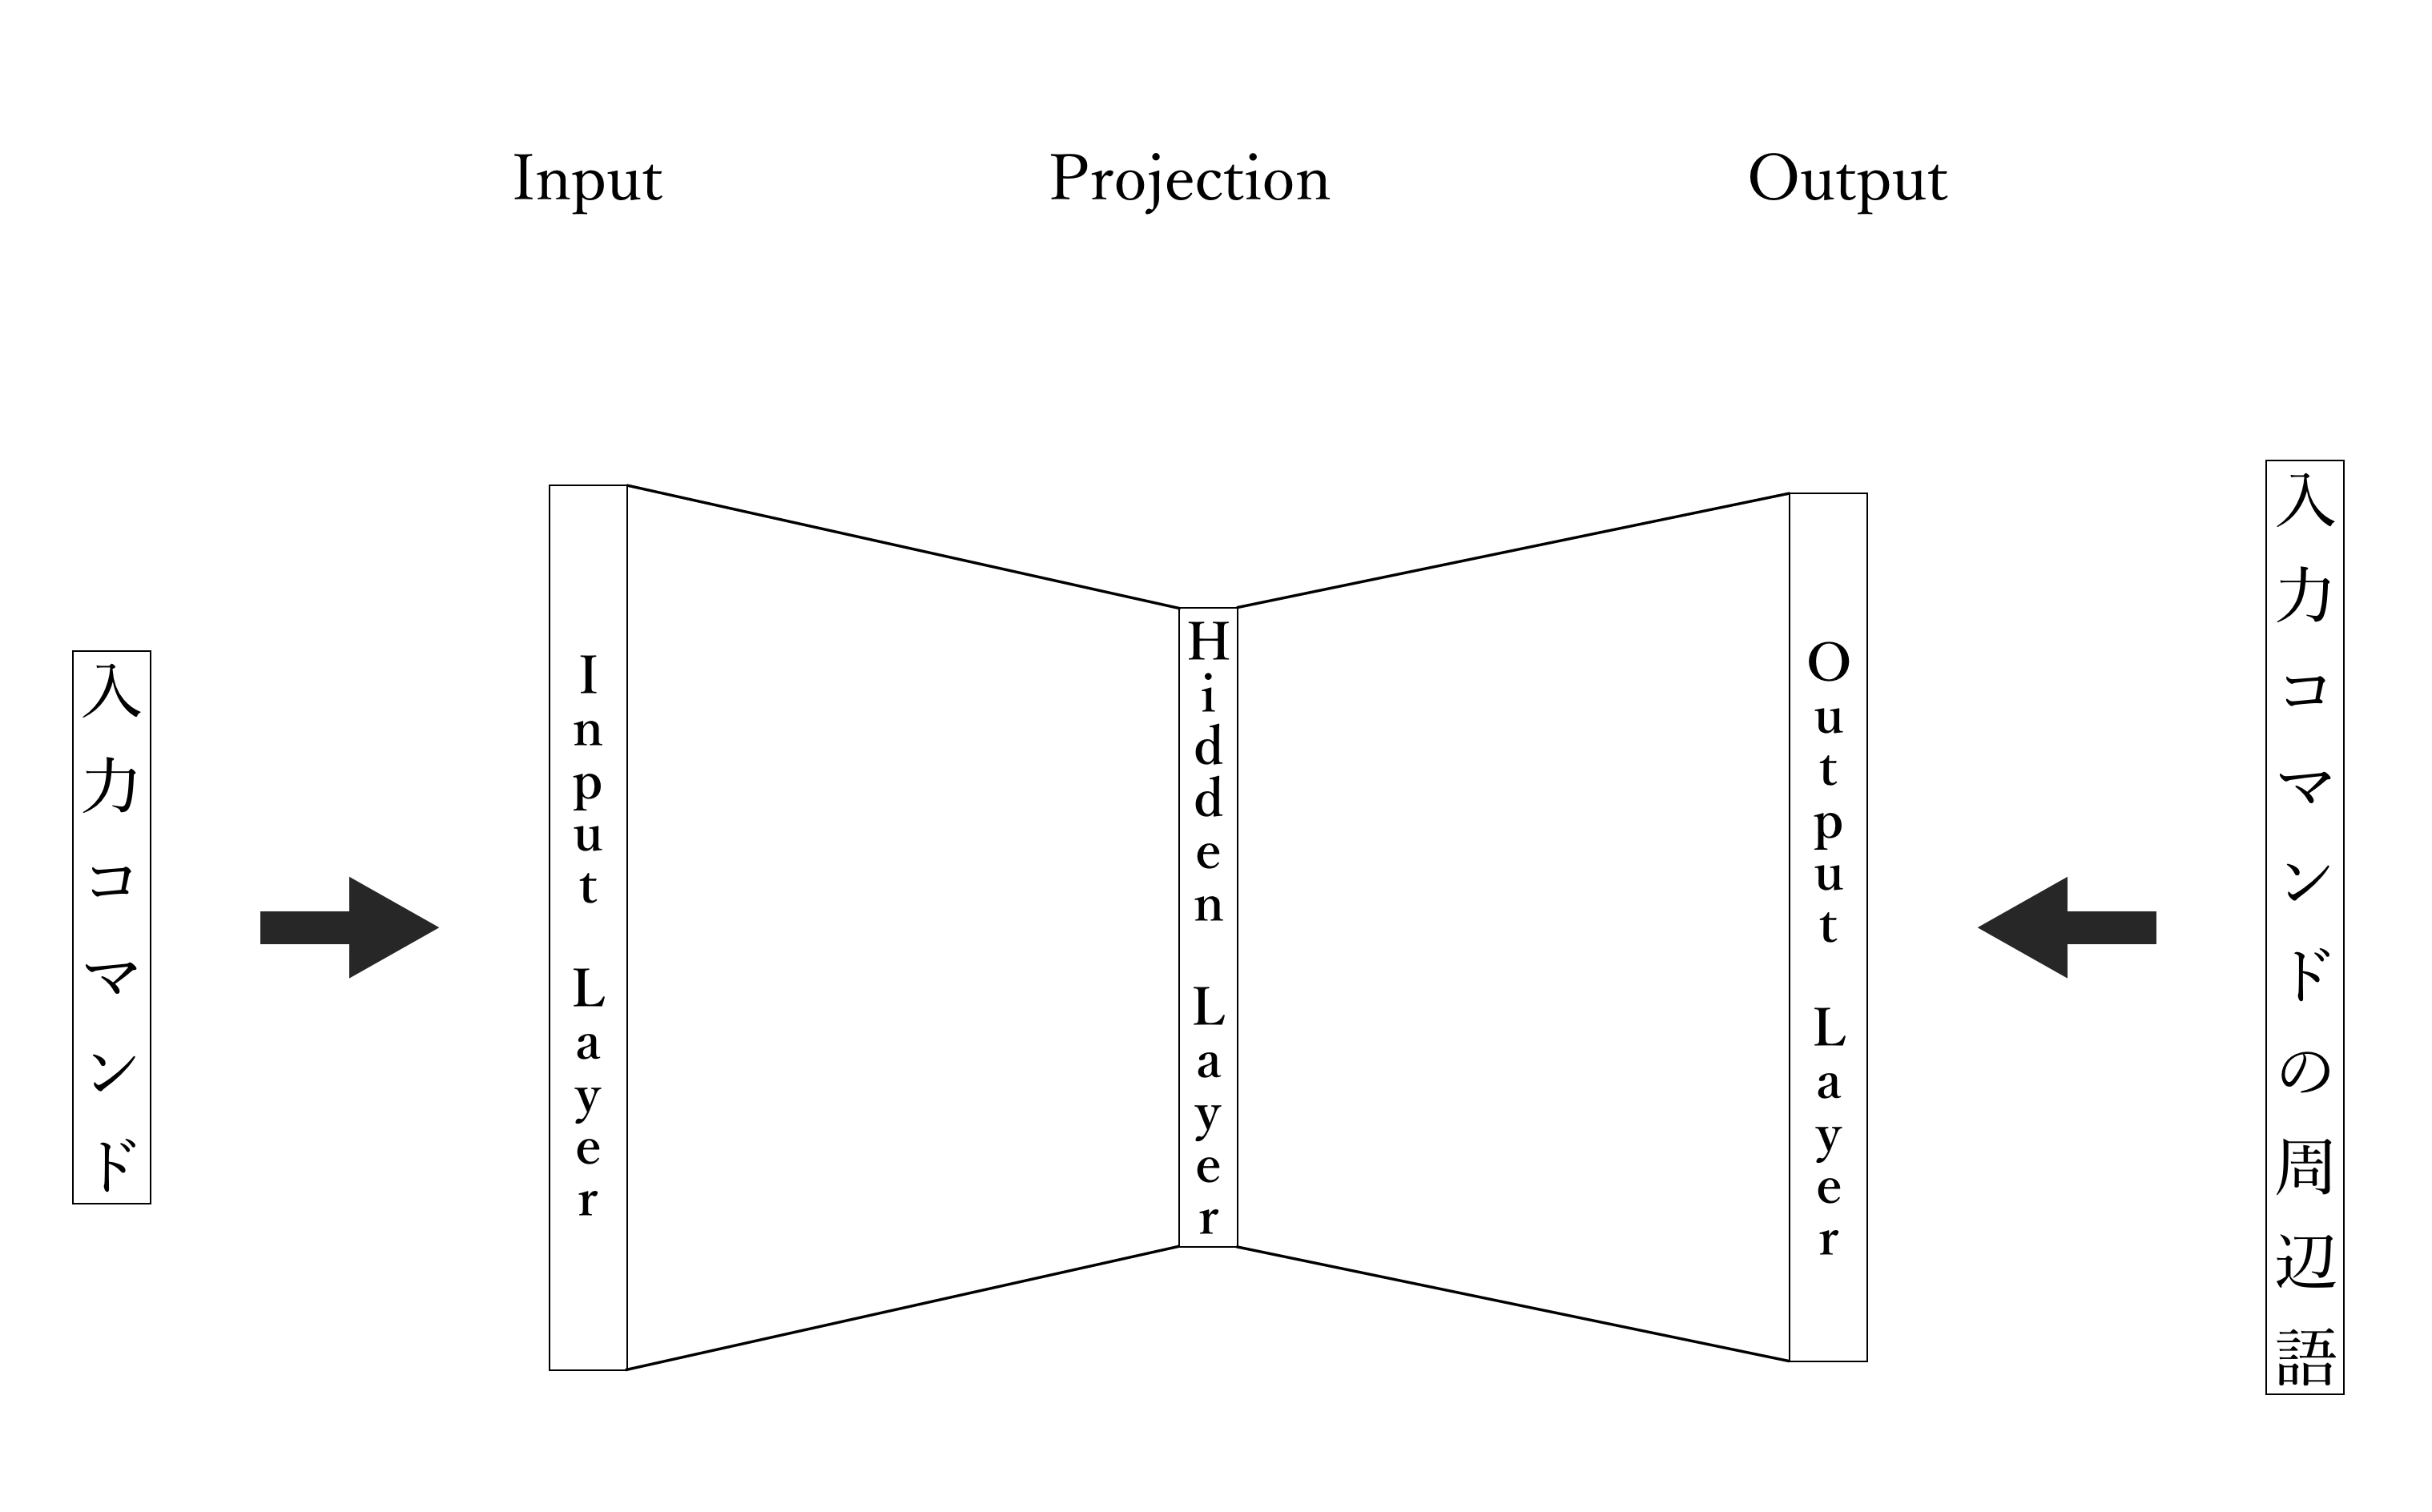
\includegraphics[width=1.0\textwidth]{figures/model.png}
    \caption{評価のフロー\cite{word2vecpaper}\cite{word2vecpaper2}}
    \label{fig:evo}
\end{figure}
\vspace{10mm}
また,このようにして純正の低対話型Honeypotの収集ログと高対話型Honeypotの収集ログに対して各々のモデルを構築する.次にこのモデルに対して,修正済みのHoneypotで収集したログを入力して,確率的にスコアリングしていくことで数値を出力する.\\

以下にこのモデルを使用した時の入力から出力のフローを図9を示す.

\begin{figure}[H]
    \centering
    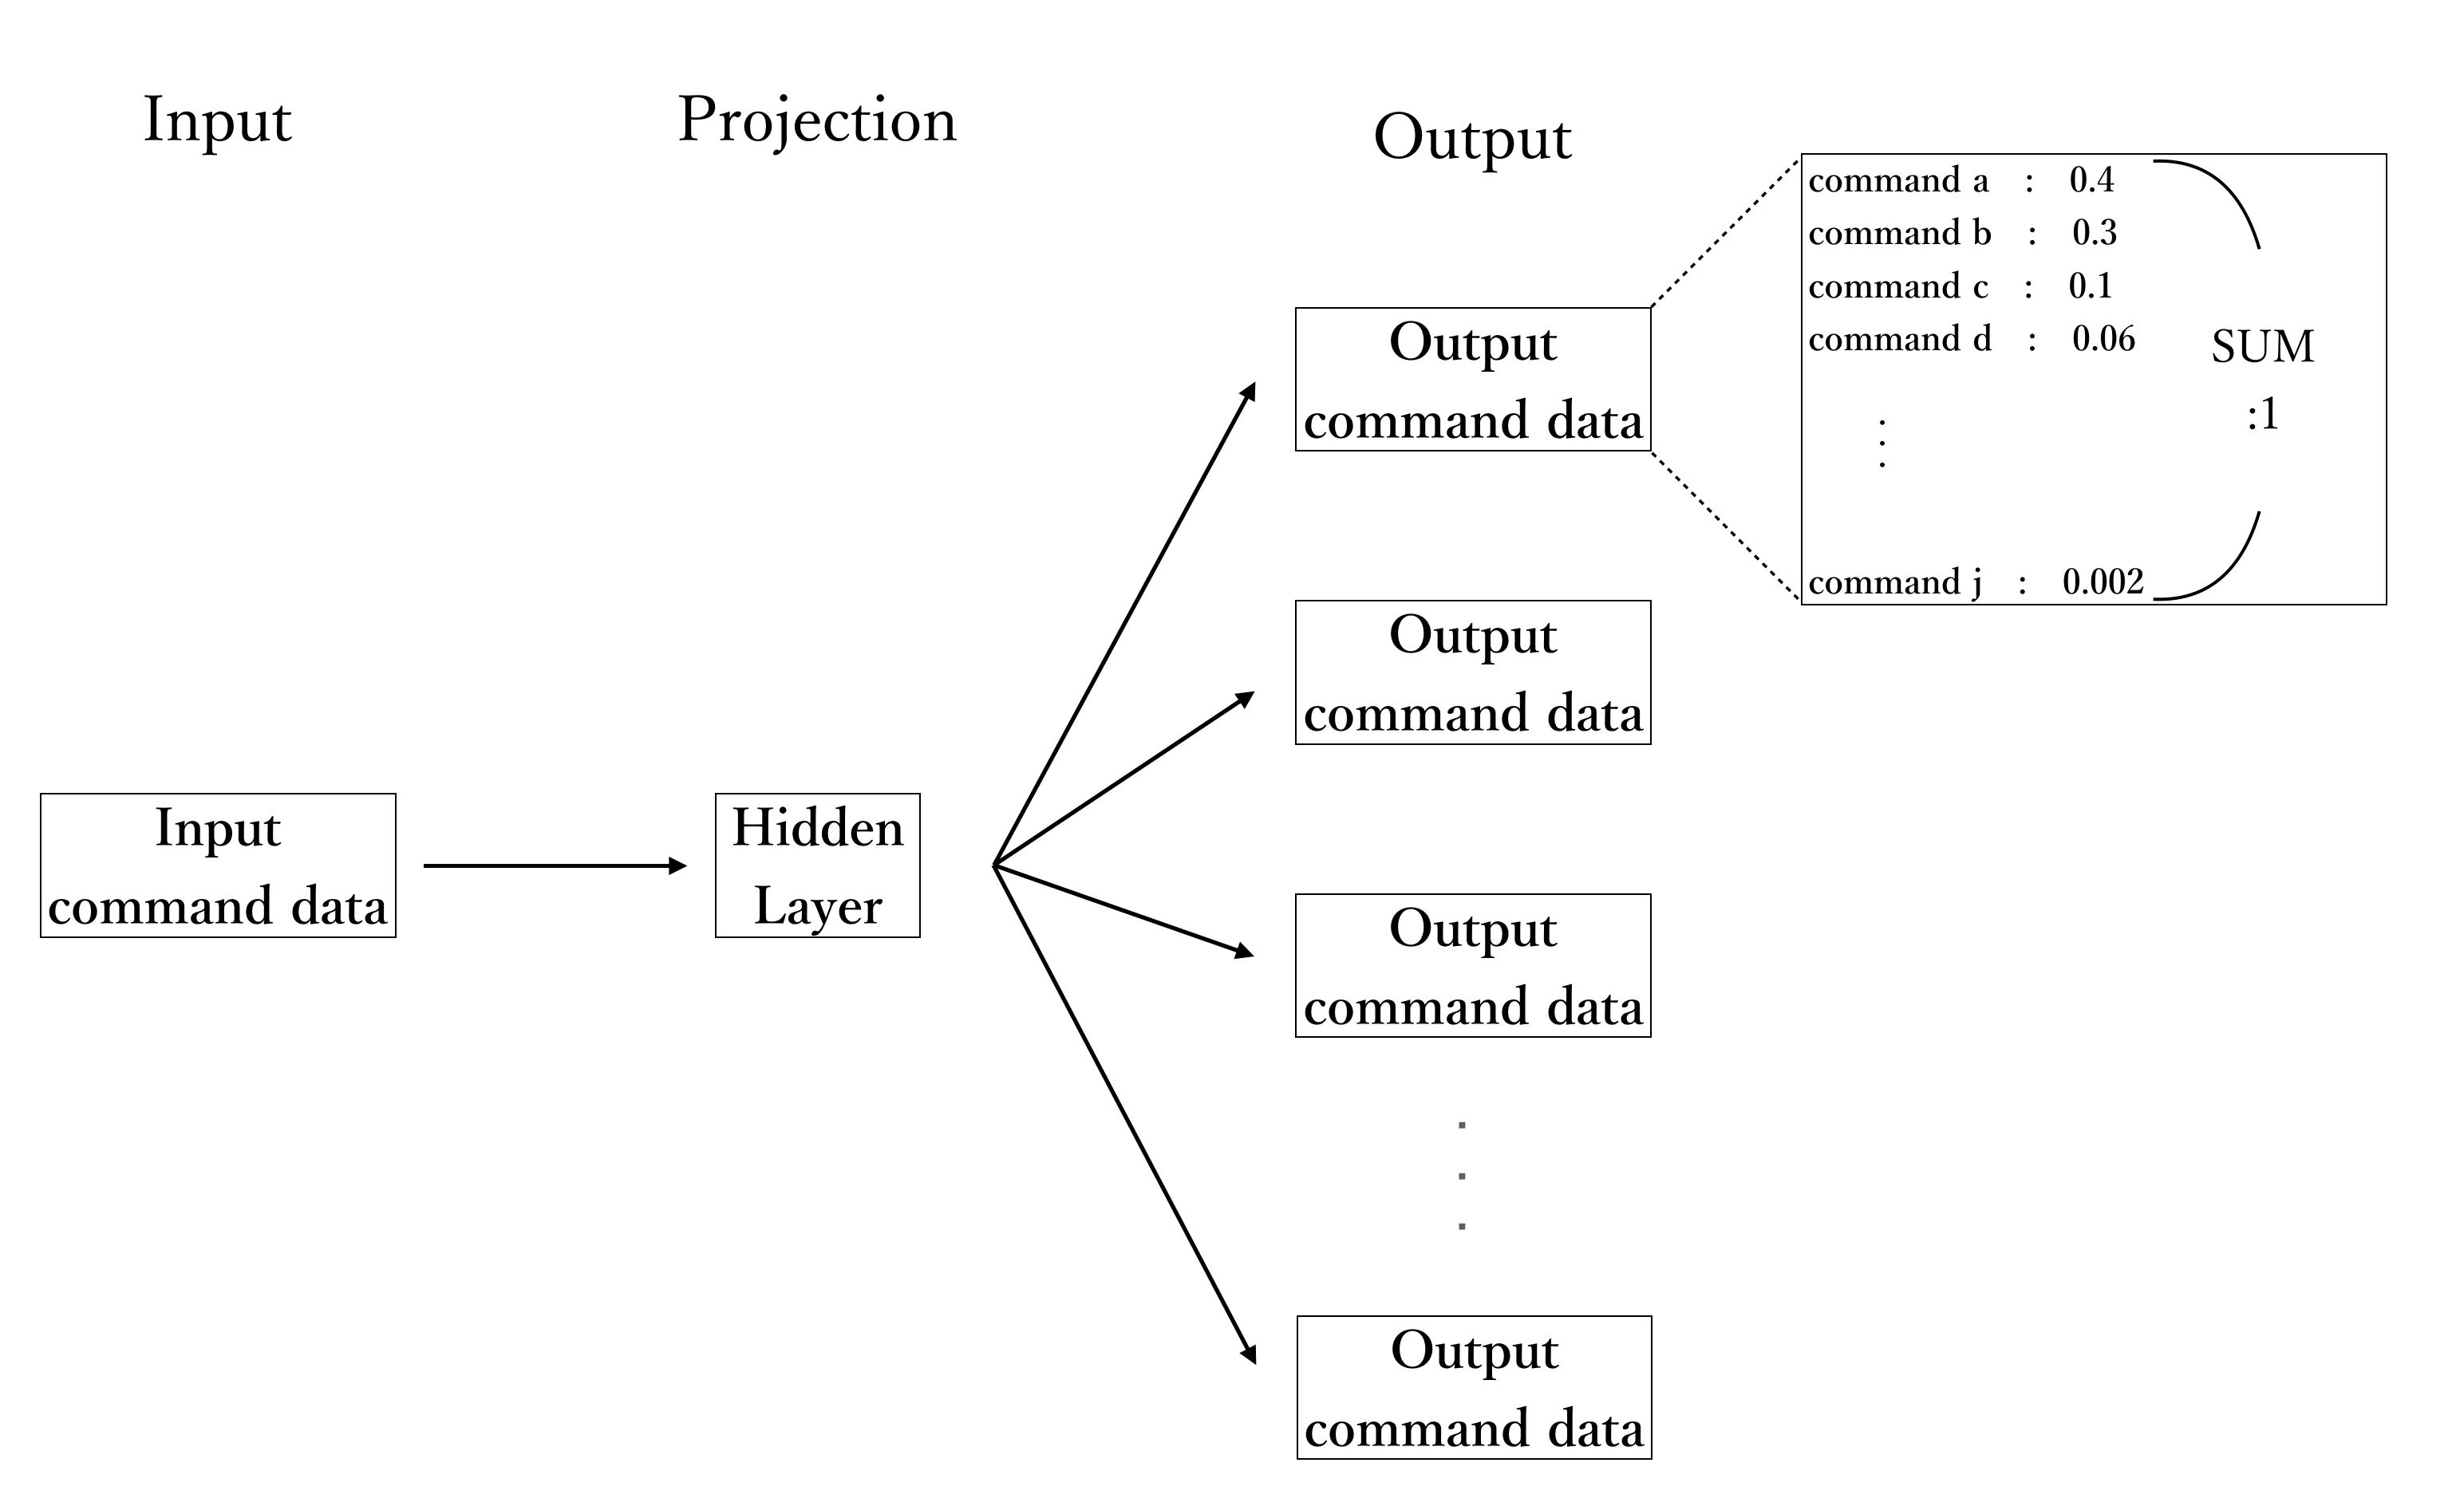
\includegraphics[width=1.0\textwidth]{figures/evalflow.png}
    \caption{評価のフロー\cite{word2vecpaper}\cite{word2vecpaper2}}
    \label{fig:evo}
\end{figure}

このようにして出力された数値を1セッションごとに平均化し,また全てのセッションにおいてもセッションごとに平均化し,全てのセッションの平均化を行うことで,純正の低対話型Honeypotの収集ログと高対話型Honeypotの収集ログとの各々で構築したモデルごとに平均値を算出する.


\subsubsubsection{コマンド群データのベクトル表現}
\label{evaluation:CommandVector}

\subsubsection{SSHの低対話型Honeypotの攻撃ログの比較}
\label{evaluation:CompareLog}



%%% Local Variables:
%%% mode: japanese-latex
%%% TeX-master: "./thesis"
%%% End:
